\newcommand{\Projekt}{LEGO GCT Pflichtenheft}

\documentclass[a4paper,12pt]{article}
\usepackage[a4paper,left=1cm,right=1cm,top=2cm,bottom=2cm]{geometry}

\usepackage[utf8]{inputenc}
\usepackage[ngerman]{babel}
\usepackage[T1]{fontenc}
\usepackage{booktabs}
\usepackage{multirow}
\usepackage{graphicx}
\usepackage{tabularx}
\usepackage{longtable}

\title{\Projekt}
\author{Caner Kara, Dennis Behrendt, Sven Wolf, Tim Sibum, Hannes Scherer,Tim Turowski}
\date{\today}

\begin{document}

\maketitle

Änderungshistorie

\begin{tabular}{|p{2cm}|p{2cm}|p{4cm}|p{8cm}|}
	\hline
	A & B & C-Spalte & C-Spalte \\ \hline
	A & B & C-Spalte & C-Spalte \\ 
	A & B & C-Spalte & C-Spalte \\ 
	A & B & C-Spalte & C-Spalte \\ 
	A & B & C-Spalte & C-Spalte \\ 
	\hline
\end{tabular}

\tableofcontents

\newpage

\section{Zielbestimmung}

Heutzutage günstig Lego-Sets zu erwerben kann auf mehreren Ebenen ein wohlüberlegtes Unterfangen sein. Welche der Lego-Händler bieten die Sets günstig an? Ist es günstiger sich die Einzelteile des Sets einzeln zu bestellen? Was ist wenn bestimmte Einzelteile nicht mehr verfügbar sind? \newline
Das Ziel des Projekts ist genau diese Fragestellungen, durch die Entwicklung eines Tools zur Ermittlung der günstigsten Anbieter, zu beantworten. Das Tool soll dabei auch in der Lage sein, abzuwägen, ob es günstiger ist, das Set oder Einzelteile zu kaufen und zu kombinieren.

\subsection{Musskriterien}
\begin{enumerate}
\item Es soll eine Datenbank mit Stücklisten und Bauteilen geben
\item Die PDF-Bauanleitungen der Lego-Sets sollen mit OCR auslesbar sein
\item Ein Crawler bezieht die Preise der unterschiedlichen Händler zur Laufzeit der Suche
\item  Ein Preisvergleich unter den Händlern, im Bezug auf Kauf eines Sets oder der jeweiligen Einzelteile, findet statt
\item Darstellung des Tools als graphische Oberfläche. (Startseite, Benuterverwaltung, Preisvergleich, Warenkorb)
\item Es soll möglich sein Benutzeraccounts anzulegen und diese zu verwalten
\item Drei feste Händler sollen beim Vergleich berücksichtigt werden
\item Auf nicht verfügbare Einzelteile sollte hinreichend hingewiesen werden.
\item Die Lieferkosten sollen beim Preisvergleich berücksichtigt werden.
\item Bei der Ausgabe des Vergleichs soll eine Verlinkung zum Produkt, sowie eine Liste der Bauteile, angezeigt werden.
\end{enumerate}

\subsection{Kannkriterien}
\begin{enumerate}
\item Plattform sollte auch auf Mobilgeräten gut dargestellt sein
\item Mehr Händler sollten noch mit aufnehmbar sein
\end{enumerate}

\subsection{Wunschkriterien}
\begin{enumerate}
\item Einzelteile die besonders selten/teuer sind sollten gesondert aufgelistet werden
\item Filterfunktion um zum Beispiel Figuren rauszufiltern
\item Sticker berücksichtigen
\item Eigene Bauanleitung auslesen lassen
\item Aktuelle Angebote hervorheben
\item Dashboard: Statistiken zum Suchverhalten unserer Benutzer / Wie erfolgreich war unser Programm?
\item Es sollte eine Funktion geben um den Warenkorb beim entsprechenden Händler automatisch befüllen zu lassen
\end{enumerate}

\subsection{Abgrenzungskriterien}
\begin{enumerate}
\item Unser Produkt wird keine Verkaufsplattform haben
\item Keine Bevorzugung von Händlern
\item Wir berücksichtigen keine nicht offiziellen Klemmbausteine
\item Website ist nur für deutschsprachige Benutzer
\item Alte Sets ohne Stückliste in der Anleitung können nicht berücksichtigt werden (2006)
\end{enumerate}

\section{Produkteinsatz}
 Das Produkt soll Benutzer bei Kaufentscheidung unterstützen, außerdem unterstützt es die Benutzer Sets zu bauen die aus irgendwelchen Gründen nicht mehr verfügbar sind.\newline
Das Tool ist für Lego-Enthusiasten und Sammler gedacht, die nach dem günstigsten Angebot suchen. Das Tool kann auch von Einzelpersonen oder Unternehmen genutzt werden, die große Mengen an Lego-Sets kaufen möchten. \newline

\section{Produktfunktionen}

\subsection{Benutzersicht}
/F10/\newline
Geschäftsprozess: Über eine Suchmaske können Lego Setnummern eingeben\newline
Vorbedingung: User befindet auf der Website des LegoGCT\newline
Nachbedingung: Nach der Eingabe wird die Datenbank auf die Existenz des Lego Sets geprüft\newline
Fehlerfall: Die Eingegebene Setnummer stimmt nicht mit einer in der Datenbank vorhanden Setnummer überein. Oder Syntaxfehler führt zur falschen Eingabe\newline
Anwender: Akteur im Kontext der Webapplikation\newline
Beschreibung: Über die Suchfunktion kann der Benutzer eine Setnummer eingeben.\newline\newline
/F20/\newline
Geschäftsprozess: Anzeigen der Historie\newline
Vorbedingung: Benutzer sollte auf der Webplattform angemeldet sein\newline
Nachbedingung: Benutzer kann sich seine persönliche Historie anzeigen lassen\newline
Fehlerfall: Benutzer hat bisher noch keinen Suchvorgang gestartet\newline
Anwender: Akteur im Kontext der Webapplikation\newline
Beschreibung: Für Angemeldete Nutzer steht die Historie vergangener Suchen zur Verfügung. Diese unterstützt den Benutzer bereits gesuchte Sets wiederzufinden.\newline\newline
/F30/\newline
Geschäftsprozess: Registrierung auf der Webplattform\newline
Vorbedingung: User befindet auf der Website des LegoGCT und hat den Registrieren Button gedrückt\newline
Nachbedingung: User konnte sich Erfolgreich registrieren lassen sein Benutzer Account wurde in einer Datenbank abgelegt\newline
Fehlerfall: E-Mail ist bereits vergeben, Datenbank ist nicht ansprechbar, Passwortsicherheit zu gering\newline
Anwender: Akteur im Kontext der Webapplikation\newline
Beschreibung: Um die vollen Funktionsumfang der Webapplikation zu nutzen. Muss der Benutzer eine Registrierung durchführen.\newline\newline
/F40/\newline
Geschäftsprozess: Anmeldung auf der Webplattform\newline
Vorbedingung: Benutzer befindet auf der Website des LegoGCT und ist ein Registrierter Nutzer\newline
Nachbedingung: Benutzer konnte sich erfolgreich an Webplattform anmelden\newline
Fehlerfall: Eine Anmeldung war nicht erfolgreich, weil Passwort und Benutzername nicht übereinstimmen oder der Benutzer noch keine Registrierung vorgenommen hat.\newline
Anwender: Akteur im Kontext der Webapplikation\newline
Beschreibung: Um die volle Funktion der Webapplikation nutzen zu können, kann sich der Benutzer an der Webplattform anmelden\newline\newline
/F50/\newline
Geschäftsprozess: Darstellung der Stücklisten\newline
Vorbedingung: Benutzer hat nach einer Setnummer gesucht, welche in der Datenbank vorhanden ist.\newline
Nachbedingung: Benutzer bekommt eine Stückliste mit Einzelteilen angezeigt \newline
Fehlerfall: Stückliste konnte nicht dargestellt werden, da zu viele Einzelteiler bei Händler nicht zur Verfügung stehen. \newline
Anwender: Akteur im Kontext der Webapplikation \newline
Beschreibung: Dem Benutzer wird eine Stückliste des Legosets ausgegeben nach dem der Benutzer gesucht hat. Die Stückliste enthält die Einzelteile mit folgenden Attributen Einzelteilnummer, Anzahl, Preis, URL \newline\newline
/F60/\newline
Geschäftsprozess: Minimieren der Stücklisten\newline
Vorbedingung: Benutzer bekommt eine Stückliste mit Einzelteilen angezeigt\newline
Nachbedingung: Benutzer bekommt nur noch den Endpreis angezeigt\newline
Fehlerfall: keinen\newline
Anwender: Akteur im Kontext der Webapplikation \newline
Beschreibung: Der Benutzer möchte eine übersichtlichere Anzeige haben und minimiert deshalb die Stückliste, um sich den Endpreis übersichtlicher darstellen zu lassen.\newline\newline
/F70/\newline
Geschäftsprozess: Anzeigen des Endpreises \newline
Vorbedingung: Benutzer \newline

\subsection{Produktfunktionen Backend} 
PDFs mit Crawler ansprechen können \newline
PDFs mittels OCR auslesen \newline
Einzelteile in Datenbank zwischenspeichern \newline
Informationen bei Händlern abfragen können \newline
Preisvergeich zwischen Sets und Einzelteilen \newline
Darstellung der Endergebnisse \newline

\section{Produktdaten}

\subsection{Bauteil}
Element-ID\newline
Name \newline

\subsection{Bauteil/Set-Preis}
Element-ID\newline
Preis\newline
Anbieter\newline
URL\newline

\subsection{Set}
Set-ID \newline
List: Element-ID \newline
Name \newline
Bool: Verfügbarkeit \newline
UVP \newline  \newline
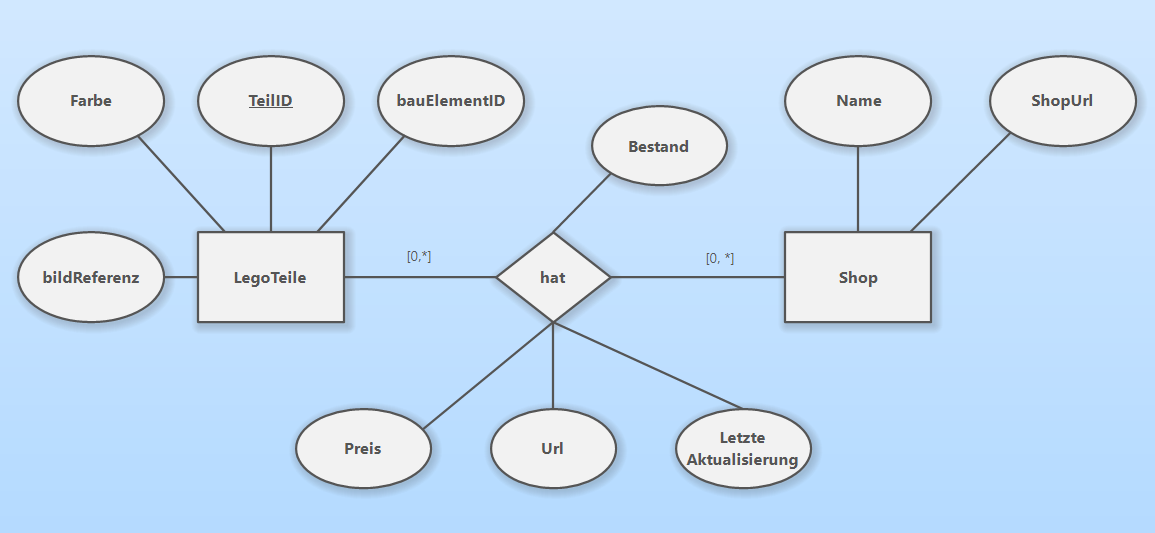
\includegraphics[width=8cm]{pictures/chen1.png} \newline  \newline
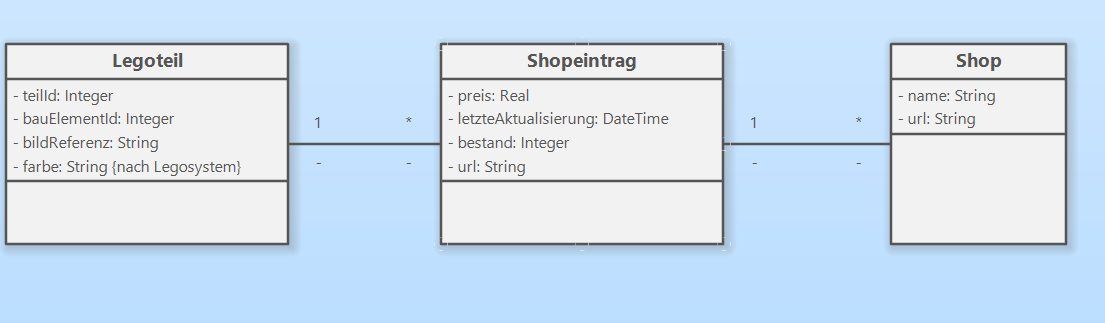
\includegraphics[width=8cm]{pictures/klassendiagramm2.png}  \newline  \newline
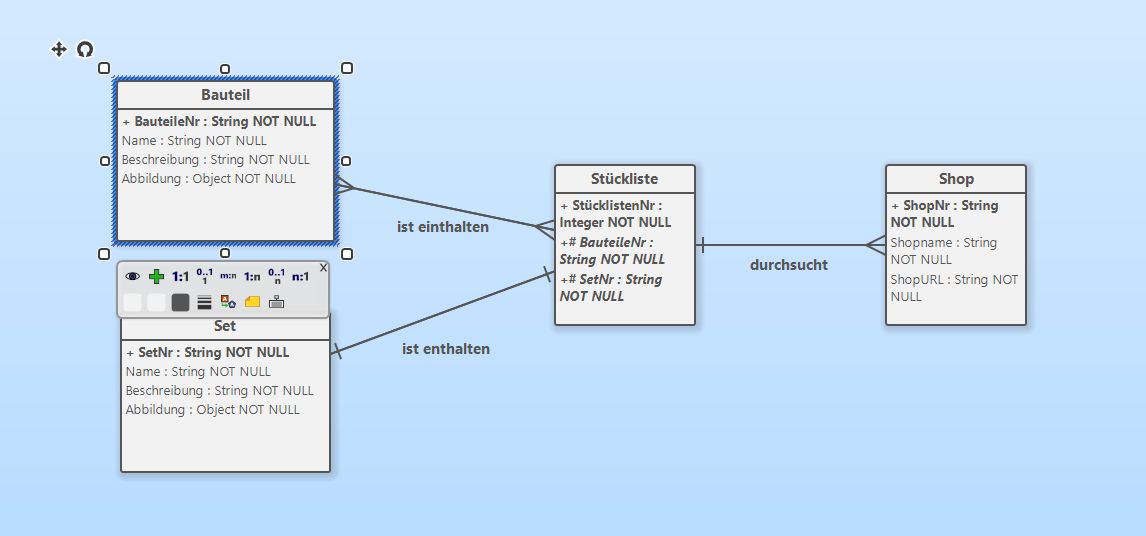
\includegraphics[width=8cm]{pictures/klassendiagramm.png} 

\section{Benutzeraccount}
Benutzername \newline
Passwort (verschlüsselt) \newline
List: Suchhistorie \newline

\section{Administrator extends Benutzeraccount}


\section{Produktleistungen}
Bestandsdatenbank soll aufgebaut werden mit Informationen aus den Anleitunge \newline
Preise sollen bei der Suche gecrawlt werden \newline
Die verwendete Datenbank muss in der Lage sein große Datenmengen zu speichern und zu verarbeiten \newline
Der Crawler soll in der Lage sein schnell Preisdaten bei den Anbietern zu crawlen, außerdem soll ein Algorithmus regelmäßig die neuen Anleitungen erkennen und dem Parser übergeben \newline

\section{Qualitätsanforderungen}
Dokumentation der Änderungshistorie \newline
Programmcode auskommentieren \newline

\section{Benutzungsoberfläche}
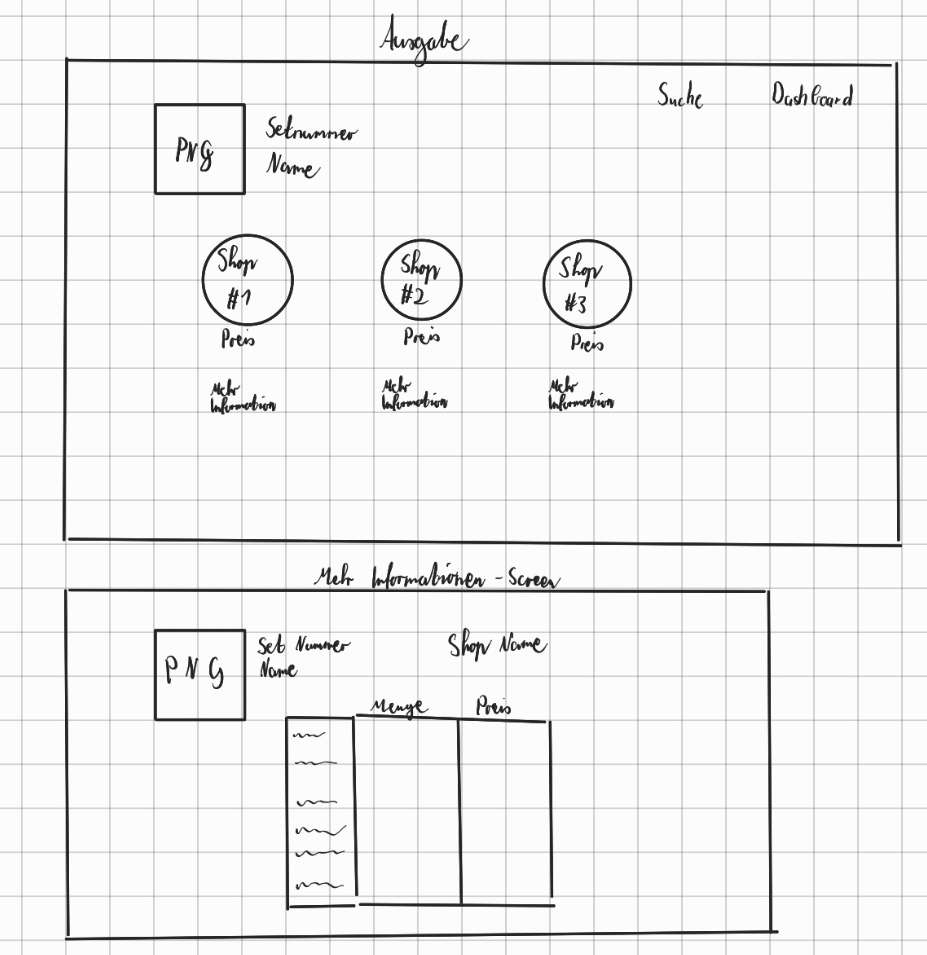
\includegraphics[width=8cm]{pictures/skizzeausgabe.jpg} \newline \newline
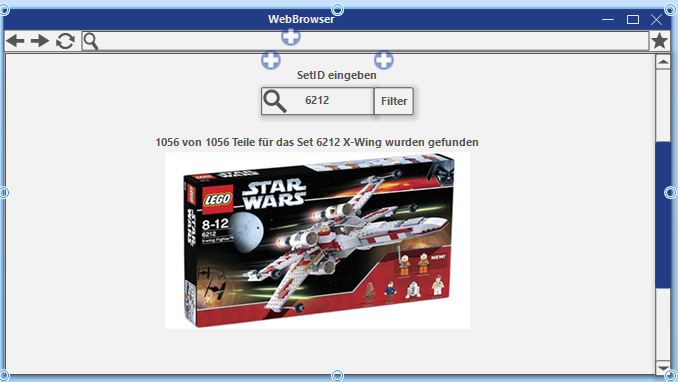
\includegraphics[width=8cm]{pictures/programmvorschau1.png}
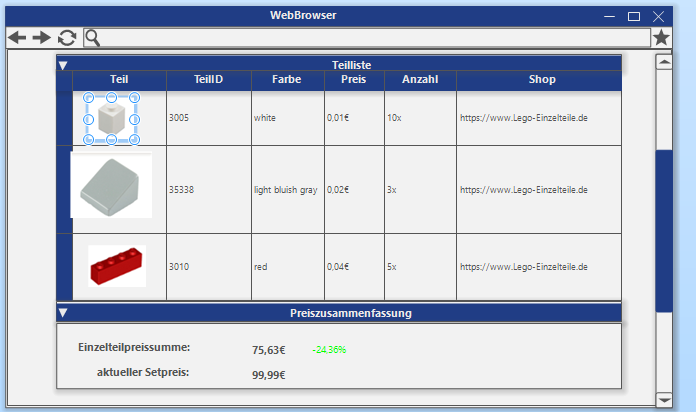
\includegraphics[width=8cm]{pictures/programmvorschau2.png} \newline \newline

\includegraphics[width=8cm]{pictures/programmvorschau3.png}

\section{Nichtfunktionale Anforderungen}
Barrierefreiheit \newline
Intuitives Design \newline
ISO Normen aus dem MCIW-Modul einhalten \newline
Revisionsinstanzen Scrum etablieren \newline
Websitendaten schützen die gecrawlt werden \newline

\section{Technische Produktumgebung}
Datenbank \newline
Crawler \newline
Webserver \newline
OCR \newline
Angular \newline
HTML \newline
CSS \newline
Python \newline
Tex \newline
Git \newline

\section{Gliederung in Teilprodukte}
Bauanleitung suchen \newline
Bauanleitung parsen \newline
Datenbank füllen \newline
Preisvergleich \newline
Ausgabe generierern \newline
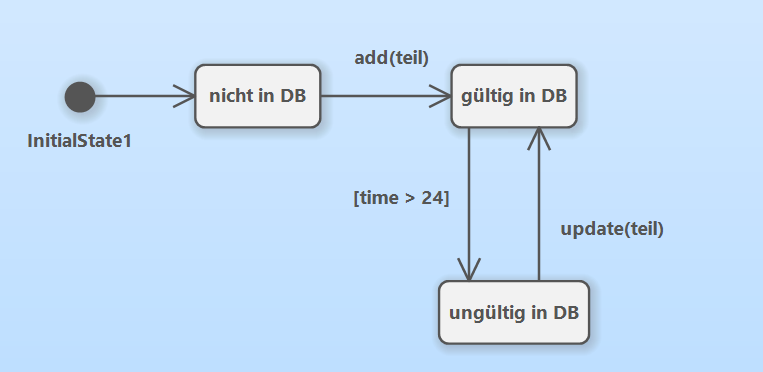
\includegraphics[width=8cm]{pictures/datenbankupdate.png} \newline  \newline
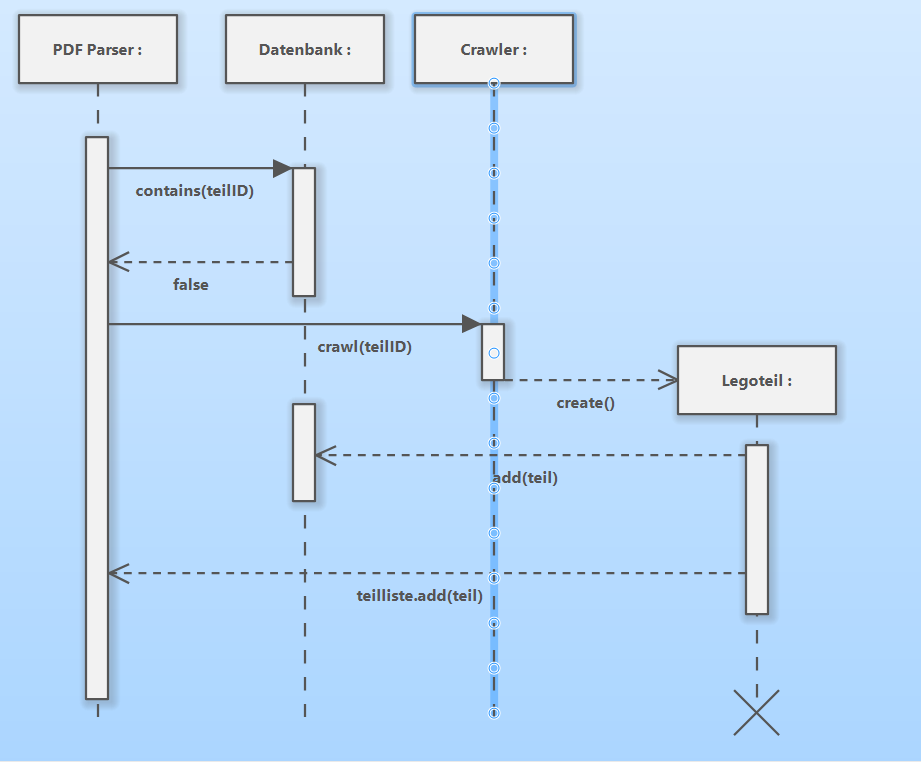
\includegraphics[width=8cm]{pictures/vorgaenge.png}


\section{Ergänzungen}
Aus rechtlichen Gründen sollen Anbieter vor dem Crawling angefragt werden \newline
Installationsanleitung und Handbuch sollen bereitgestellt werden \newline

\section{Globale Testfälle}
Set händisch recherchieren, um Soll-Wert für Unit-Test zu ermitteln und mit Algortihmusausgabe testen \newline
Gesucht wird ein Lego-Set, dessen Bauanleitung keine Stückliste besitzt -> Meldung besagt, dass die Applikation dieses Set nicht unterstützt, der Link zur Bauanleitung wird allerdings ausgegeben \newline
Gültige Set-ID wird gesucht -> Die Applikation gibt eine Stückliste aus, pro Webshop einen Preis für das fertige Set und einen Preis für den Kauf der Einzelteile, pro Shop \newline
Ungültige Set-ID wird gesucht -> Eine Fehlermeldung wird ausgegeben, die besagt dass zu dieser Setnummer kein Lego Set existiert oder aufgrund von Neuheit noch nicht in der Datenbank enthalten ist \newline
Historie anzeigen, obwohl noch kein Suchvorgang ausgeführt wurde -> Die Historie ist leer \newline
E-Mail Adresse beim Registrieren schon vergeben -> Dem Benutzer wird mitgeteilt, dass zu dieses Email-Adresse bereits ein Benutzerkonto besteht \newline
Datenbank während Registrierung nicht ansprechbar -> Der Benutzer wird gebeten seine Aktion später nochmal zu wiederholen, da ein Fehler aufgetreten ist \newline
Passwort für Benutzerkonto ist zu unsicher -> Der Benutzer wird aufgefordert ein neues Passwort einzugeben, welches eine höhere Sicherheitsstufe besitzt \newline
Benutzername und Passwort stimmen bei Anmeldung nicht überein -> Dem Benutzer wird mitgeteilt, dass das Passwort nicht zum Benutzernamen passt und er es nochmal versuchen soll \newline
Benutzername bei Anmeldung noch nicht Registriert -> Eine Meldung wird ausgegeben, dass der Benutzername noch keinem Benutzerkonto zugeteilt ist \newline
Bestimmt viele Einzelteile sind bei Händlern nicht verfügbar -> Eine Mitteilung 

\end{document}